% !TeX spellcheck = de_DE
% Document setup
%\documentclass[AMdocument]{AMlatex}%             german version
\documentclass[AMdocument,optGerman]{AMlatex}% english version
%
% Set paths
%\graphicspath{{./_pic/}}
%\addbibresource{./_aux/literature.bib}
%
\usepackage{amsmath}
\usepackage{booktabs}
\usepackage{chngcntr}
% 

% Here bigins
\begin{document}%
%
\AMTitlePageDefault{Roboterdynamik - Praktikum WS17/18}{Modulprüfstand - Gruppe3}{Qiming Yu, Marc Schmid, Katharina Wurtinger}%  
%\AMTitlePageDefault{Title}{Subtitle}{Author}%  
%
\numberwithin{equation}{section}
\numberwithin{table}{section}
\numberwithin{figure}{section}

\section{Simulation}
%
\subsection{Steuerbedingung}
%
Aufgabe 1: $$ \quad U_{d} = -p\omega_{m}L_{q}I_{q} $$
%
\subsection{Gegenspannungskompensation}
%
Aufgabe 2: $$ \quad U_{q,komp} = U_{q} - \hat{U}_{q} = p\omega_{m}\psi_{PM}  $$
%
\subsection{Stromregler}
%
Aufgabe 3.1 
\begin{align*}
\hat{U}_{q}(s) &= (sL_{q} + R)I_{q}(s) \\
\Rightarrow H_{el}(s) &= \dfrac{I_{q}(s)}{\hat{U}_{q}(s)} = \dfrac{\frac{1}{R}}{1+s\frac{L_{q}}{R}} 
\end{align*}
Das ist ein PT-1 Glied.\\

%
Aufgabe 3.2
\begin{align*}
sT_{LV}(s)\hat{U}_{q}(s) + \hat{U}_{q}(s) = \hat{U}_{q,ideal}(s) \\
\Rightarrow H_{LV}(s) = \dfrac{\hat{U}_{q}(s)}{\hat{U}_{q,ideal}(s)} = \dfrac{1}{1+sT_{LV}}
\end{align*}
%
Aufgabe 3.3
$$ G_{I}(s) = \dfrac{I_{q}(s)}{\hat{U}_{q,ideal}(s)} = H_{el}(s)H_{LV}(s) =  \dfrac{\frac{1}{R}}{(1+s\frac{L_{q}}{R})(1+sT_{LV})} $$
%
Aufgabe 3.4
$$ R_{I}(s) = \dfrac{\hat{U}_{q}(s)}{I_{q,soll}(s) - I_{q}(s)} = V_{IR}\dfrac{1+sT_{In}}{sT_{In}} $$
$$ V_{IR} = \dfrac{T_{1}}{2T_{\sigma}V_{s}} = \dfrac{L_{q}}{2T_{LV}}, \quad T_{In} = T_{1} = \dfrac{L_{q}}{R} $$
%

\clearpage

Aufgabe 3.5
\begin{figure}[htb]%
	\centering%
	% Including .pdf
	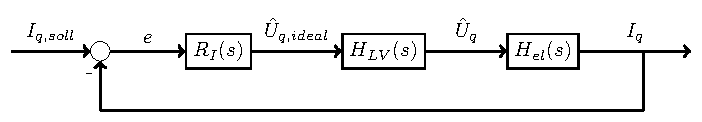
\includegraphics[width=120mm]{Stromregler}\par%
	%
	\caption{Blockschaltbild des geschlossenen Stromregelkreises}%
	\label{fig:MyImage}%
\end{figure}%
\\
%
Aufgabe 3.6
$$(I_{q,soll}(s) -I_{q}(s))R_{I}(s)G_{I}(s) = I_{q}(s)$$
$$\Rightarrow I_{q,soll}(s)R_{I}(s)G_{I}(s) = \left[ 1+R_{I}(s)G_{I}(s)\right]I_{q}(s)$$
$$\Rightarrow K_{I}(s) = \dfrac{I_{q}(s)}{I_{q,soll}(s)} = \dfrac{1}{1+s2T_{LV}+s^{2}2T_{LV}^{2}}$$

\subsection{Drehzahlregler}
Aufgabe 4.1
\begin{align*}
Js\omega_{m}(s) &= \frac{2}{3}p\psi_{PM}I_{q} \\
\Rightarrow \quad H_{\omega}(s) &= \dfrac{\omega_{m}(s)}{I_{q}(s)} = \dfrac{\frac{2}{3}p\psi_{PM}}{Js}
\end{align*}
%
Aufgabe 4.2
$$ G_{\omega}(s) = \dfrac{\omega_{m}(s)}{I_{q,soll}(s)} = K_{I}(s)H_{\omega}(s) =  \dfrac{\frac{2}{3}p\psi_{PM}}{Js(1+s2T_{LV})} $$
%
Aufgabe 4.3
$$ R_{\omega}(s) = \dfrac{I_{q,soll}(s)}{\omega_{m,soll}(s) - \omega_{m}(s)} = V_{\omega R}\dfrac{1+sT_{\omega n}}{sT_{\omega n}} $$
$$ V_{\omega R} = \dfrac{T_{1}}{2T_{\sigma}V_{s}} = \dfrac{J}{6p\psi_{PM}T_{LV}}, \quad T_{\omega n} = 4T_{\sigma} = 8T_{LV} $$
%
Aufgabe 4.4
\begin{figure}[htb]%
	\centering%
	% Including .pdf
	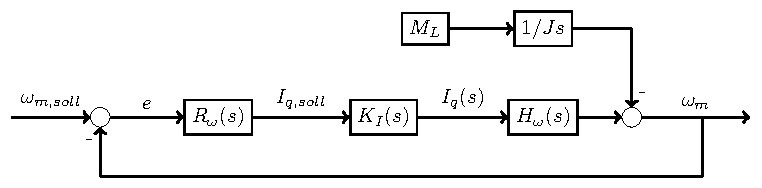
\includegraphics[width=120mm]{Drehzahlregler}\par%
	%
	\caption{Blockschaltbild des geschlossenen Drehzahlregelkreises}%
	\label{fig:MyImage}%
\end{figure}%
\\
% 
Aufgabe 4.5
$$ K_{\omega}(s) = \dfrac{\omega_{m}(s)}{\omega_{m,soll}(s)} = \dfrac{1+s8T_{LV}}{1+s8T_{LV}+s^{2}32T_{LV}+s^{4}64T_{LV}} $$
%
\subsection{Positionsregler}
% 
Aufgabe 5.1
$$ H_{\psi}(s) = \dfrac{\psi_{m}(s)}{\omega_{m}(s)} = \frac{1}{s} $$
%
Aufgabe 5.2
$$ G_{\psi}(s) = \dfrac{\psi_{m}(s)}{\omega_{m,soll}(s)} = H_{\psi}(s)K_{\omega}(s) = \dfrac{1}{s(1+s8T_{LV})} $$
Variante 1: 
$$ R_{\psi}^{P}(s)=V_{\psi R}^{P} $$
$$ V_{\psi R}^{P} = \dfrac{1}{16T_{LV}} $$
Variante 2: 
$$ R_{\psi}^{P}(s)=V_{\psi R}^{PI}\dfrac{1+sT_{\psi n}^{PI}}{sT_{\psi n}^{PI}} $$
$$ V_{\psi R}^{PI} = \dfrac{1}{16T_{LV}}, \quad T_{\psi n}^{PI} = 32T_{LV} $$
%
Aufgabe 5.3
\begin{figure}[htb]%
	\centering%
	% Including .pdf
	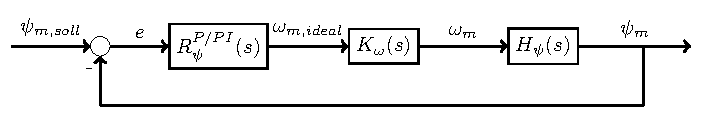
\includegraphics[width=120mm]{Positionsregler}\par%
	%
	\caption{Blockschaltbild des geschlossenen Positionsregelkreises}%
	\label{fig:MyImage}%
\end{figure}%

\subsection{Blockschaltbild Kaskadenregelung}
Aufgabe 6
\begin{figure}[htb]%
	\centering%
	% Including .pdf
	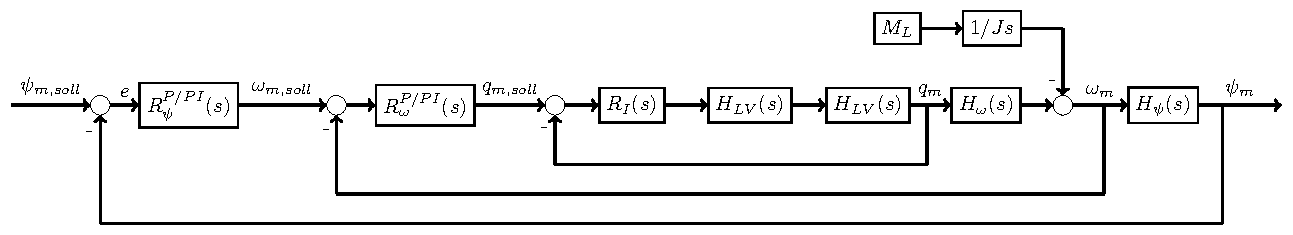
\includegraphics[width=140mm]{Kaskadenregelung}\par%
	%
	\caption{das Gesamt-Blockschaltbild der Kaskadenregelung}%
	\label{fig:MyImage}%
\end{figure}%

\end{document}%
%
%
